\documentclass[12pt,a4paper]{article}
\usepackage{algorithm}
\usepackage{algpseudocode}
\usepackage{listings}
\usepackage{marvosym}
\usepackage{wasysym}
\usepackage{marvosym}
\usepackage{xcolor}
\usepackage{graphicx}
\usepackage{tikz}
\usepackage{tikz-uml}
\usetikzlibrary{positioning,shapes,arrows}
\usetikzlibrary{automata,positioning,shapes,arrows,backgrounds,fit}

\author{Sujit Chakrabarti}
\title{Object Oriented Programming}
\date{}
\begin{document}
\definecolor{lightblue}{rgb}{0.8,0.93,1.0} % color values Red, Green, Blue
\definecolor{Blue}{rgb}{0,0,1.0} % color values Red, Green, Blue
\definecolor{Red}{rgb}{1,0,0} % color values Red, Green, Blue
\definecolor{Purple}{rgb}{0.5,0,0.5}
\definecolor{Pink}{rgb}{0.7,0,0.2}

\newcommand{\highlight}[1]{{\color{Red}(#1)}}
\newcommand{\comment}[1]{{\color{Blue}#1}}

\lstset{
	language = Java,
	basicstyle = \ttfamily\small,
	stringstyle = \ttfamily,
	keywordstyle=\color{black},
	identifierstyle=\color{black},
	frameround=tttt,
	numbers=none,
	showstringspaces=false
}

\maketitle

\section{Inheritance}
Let's return to our shape classes by implementing a \lstinline@Rectangle@ class.

\begin{figure}[H]
\begin{lstlisting}[frame=single]

class Rectangle {

  protected final float length;
  private final float breadth;

  public Rectangle(float l, float b) {
    this.length = l;
    this.breadth = b;
  }

  public float area() {
    return this.length * this.breadth;
  }

}
\end{lstlisting}
\caption{A rectangle class}
\label{f:rec1}
\end{figure}

The code in fig.~\ref{f:rec1} can be tested as follows:
\begin{lstlisting}[frame=single]
public class Geometry2 {

  public static void main(String[] a) {
    Rectangle r = new Rectangle(10, 20);
    System.out.println("area = " + r.area());
  }
}
\end{lstlisting}

Next, let's also add a \lstinline@Square@ class to the code.
\begin{figure}[H]
\begin{lstlisting}[frame=single]

class Square {

  private final float length;
  public Square(float l) {
    this.length = l;
  }

  public float area() {
    return this.length * this.length;
  }
}
\end{lstlisting}
\caption{A square class}
\label{f:sq1}
\end{figure}

The code in fig.~\ref{f:sq1} can be tested as follows:
\begin{lstlisting}[frame=single]
public class Geometry2 {

  public static void main(String[] a) {
    Rectangle r = new Rectangle(10, 20);
    System.out.println("area = " + r.area());
    Square s = new Square(200);
    System.out.println("area = " + s.area());
  }
}
\end{lstlisting}

The \lstinline@Rectangle@ and \lstinline@Square@ classes fig.~\ref{f:rec1} and fig.~\ref{f:sq1} aren't similar by coincidence. The fact is, a square is a rectangle with its length equal to its breadth. Unfortunately, the code here doesn't capture this fact. It would be nice if we could make this knowledge an explicit part of our code. Does Java allow us to do that? Yes, it does! 
\begin{figure}[H]
\begin{lstlisting}[frame=single]

class Square extends Rectangle {

  private final float length;
  public Square(float l) {
    this.length = l;
  }
  
  public float area() {
    return this.length * this.length;
  }
}
\end{lstlisting}
\caption{\lstinline@Square@ class declared a sub-class of \lstinline@Rectangle@}
\label{f:sq2}
\end{figure}

The code in fig.~\ref{f:sq2} modifies that in fig.~\ref{f:sq1} by declaring \lstinline@Square@ as a sub-class of \lstinline@Rectangle@, by using the \lstinline@extends@ keyword as shown. This is good. But it doesn't do much functionally. However, following version of the \lstinline@Square@ class does the real magic!
\begin{figure}[H]
\begin{lstlisting}[frame=single]

class Square extends Rectangle {
  public Square(float l) {
    super(l, l);
  }
}
\end{lstlisting}
\caption{\lstinline@Square@ class declared a sub-class of \lstinline@Rectangle@}
\label{f:sq3}
\end{figure}

Several lines from the \lstinline@Square@ have been reduced. Does this code even compile? Sure enough, it does! In particular, the call to \lstinline@s.area()@ from the \lstinline@main@ method compiles in spite of there being no \lstinline@area@ method anymore in the \lstinline@Square@ class. And if you run the code, it seems to work just as fine as before, giving the same result. How could this happen?

The reason for this is: \lstinline@Square@ being the \emph{child} of the \lstinline@Rectangle@ class, \emph{inherits} all its properties. This is called \emph{inheritance}, the most important feature of all object oriented programming languages. We say that:
\begin{itemize}
	\item \lstinline@Square@ inherits from \lstinline@Rectangle@.
	\item \lstinline@Square@ is the sub-class/child-class/sub-type/child-type/derived-class of \lstinline@Rectangle@.
	\item \lstinline@Rectangle@ is the super-class/parent-class/super-type/parent-type of \lstinline@Square@.
\end{itemize} 

Thus, \lstinline@area@ method in \lstinline@Rectangle@ also becomes a property of \lstinline@Square@. But this \lstinline@area@ method needs the \lstinline@length@ and \lstinline@breadth@ attributes of \lstinline@Rectangle@ to be set to the correct values (in this case, equal to the \lstinline@length@ attribute (now deleted) of the \lstinline@Square@ class). Where and how does this happen?

It happens in the constructor of \lstinline@Square@ class, when \lstinline@super(l, l)@ executes. To understand what this does consider the pictures in fig.~\ref{f:sup}.
\begin{figure}[H]
\begin{center}
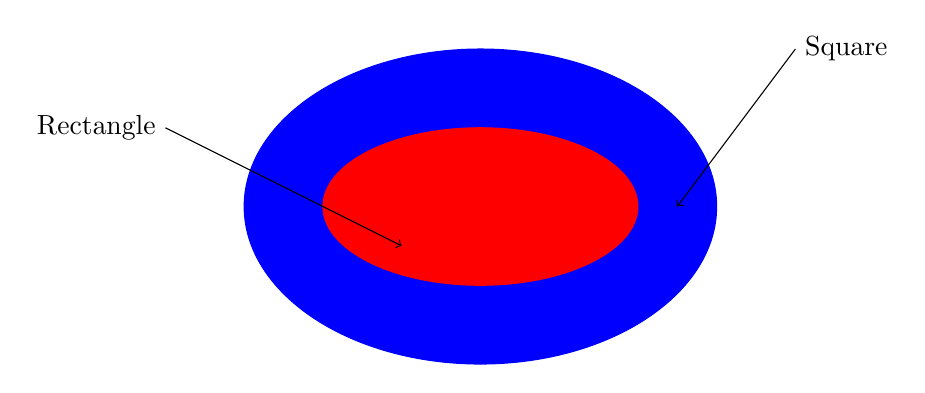
\begin{tikzpicture}
\draw[blue, fill=blue] (0,0) ellipse (3cm and 2cm);
\draw[red, fill=red] (0,0) ellipse (2cm and 1cm);

\draw[->] (4cm, 2cm) node[right]{Square} -- (2.5cm, 0cm);
\draw[->] (-4cm, 1cm) node[left]{Rectangle} -- (-1cm, -0.5cm);
\end{tikzpicture}

\end{center}
\caption{\lstinline@Square@ object with an object of \lstinline@Rectangle@ embedded within itself}
\label{f:sup}
\end{figure}

Each object of a sub-class can be visualised as embedding within it an object of its super-class. Thus, an object of \lstinline@Square@ class has within it an object of \lstinline@Rectangle@ as shown in fig.~\ref{f:sup}. During the construction of a sub-class object, the first step to complete is the construction of the embedded super-class object. The call to \lstinline@super@ method does precisely this. It calls the constructor of the super-class with the given arguments, in this case \lstinline@l@ and \lstinline@l@ (\lstinline@l@ being the parameter to \lstinline@Square@'s constructor).

This initialises the embedded \lstinline@Rectangle@ to have its \lstinline@length@ and \lstinline@breadth@ attributes both set to the argument passed to the constructor to \lstinline@Square@. Thus, a subsequent call to \lstinline@s.area@ in the \lstinline@main@ method calls the \lstinline@area@ method of the embedded \lstinline@Rectangle@ object. This, in turns returns the product of \lstinline@length@ and \lstinline@breadth@ attributes (which, remember, are equal to each other) thus giving us the correct \lstinline@area@ of the \lstinline@Square@.

So, \lstinline@super@ is a new keyword we have learned, it used in the context of a sub-class, is essentially a reference to the embedded instance of the superclass.  

Can we derive further classes from \lstinline@Square@? Yes, and we present an example in fig.~\ref{f:pt}.
\begin{figure}[H]
\begin{lstlisting}[frame=single]

class Point extends Square {
  public Point() {
    super(0);
  }
}
\end{lstlisting}
\caption{\lstinline@Square@ class declared a sub-class of \lstinline@Rectangle@}
\label{f:pt}
\end{figure}

Again, a very rudimentary class, with hardly any code! It just creates the new type \lstinline@Point@ as a sub-type of \lstinline@Square@, making point a special type of square with zero length, which is indeed a reasonable way to look at things.

The code in fig.~\ref{f:pt} can be tested with the following lines added to the \lstinline@main@ method:
\begin{lstlisting}[frame=single]
    Square p = new Point();
    System.out.println("area = " + p.area());
\end{lstlisting}

This works just smoothly, giving us the expected results:
\begin{lstlisting}[frame=single]
area = 0.0
\end{lstlisting}

Indeed, a point is a square (and hence a rectangle) with zero area. Pictorially, the scenario can be depicted as in fig.~\ref{f:sup2}.
\begin{figure}[H]
\begin{center}
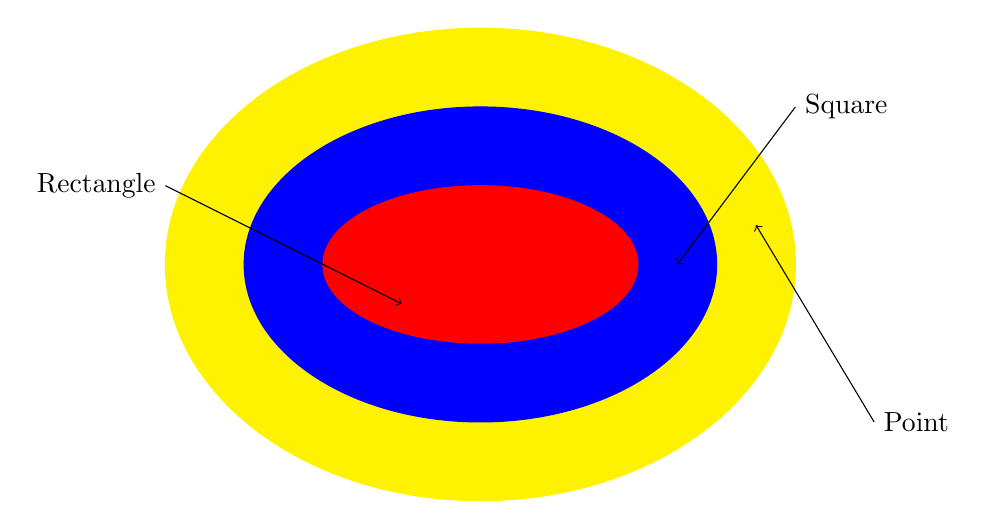
\begin{tikzpicture}
\draw[yellow, fill=yellow] (0,0) ellipse (4cm and 3cm);
\draw[blue, fill=blue] (0,0) ellipse (3cm and 2cm);
\draw[red, fill=red] (0,0) ellipse (2cm and 1cm);

\draw[->] (5cm, -2cm) node[right]{Point} -- (3.5cm, 0.5cm);
\draw[->] (4cm, 2cm) node[right]{Square} -- (2.5cm, 0cm);
\draw[->] (-4cm, 1cm) node[left]{Rectangle} -- (-1cm, -0.5cm);
\end{tikzpicture}

\end{center}
\caption{\lstinline@Point@ object with an object of \lstinline@Square@ embedded within itself}
\label{f:sup2}
\end{figure}

\subsection{Access Specifier \lstinline@protected@}
Any method from within \lstinline@Square@ class won't be able to access \lstinline@Rectangle@'s \lstinline@length@ attribute directly. This may be OK sometimes, but sometimes this may be too restrictive. For example, the following piece of code
\begin{lstlisting}[frame=single]
  public float circumference() {
    return 4.0f * this.length;
  }
\end{lstlisting}
if added to the \lstinline@Square@ class would lead to a compilation error:
\begin{lstlisting}[frame=single]
 error: length has private access in Rectangle
    return 4.0f * this.length;
\end{lstlisting}


In other words, the designer of the \lstinline@Rectangle@ class may want the implementers of its sub-classes to have direct access to \lstinline@length@. One option would be to turn \lstinline@length@ into a \lstinline@public@ attribute. This would work, but this is an overkill, and too permissive. We would like to tune the visibility of \lstinline@length@ to just the level where the sub-classes have direct access to it, but it remains invisible to any other class in the program. For this we use the \lstinline@protected@ access specifier:
\begin{lstlisting}[frame=single]
  protected float length;
\end{lstlisting}

With this, it is possible to write code within \lstinline@Square@ class that directly refers to \lstinline@length@. For instance, the code added to \lstinline@Square@ above, now works!

\section{Polymorphism}

\begin{figure}[H]
\begin{lstlisting}[frame=single]
  public static void main(String[] a) {
    Rectangle r = new Rectangle(10, 20);
    System.out.println("area = " + r.area());
    r = new Square(10);
    System.out.println("area = " + r.area());
    r = new Point();
    System.out.println("area = " + r.area());
  }
\end{lstlisting}
\caption{\lstinline@Square@ class declared a sub-class of \lstinline@Rectangle@}
\label{f:poly}
\end{figure}

Consider the modified \lstinline@main@ method shown in fig.~\ref{f:poly}. The notable point here is that the variable \lstinline@r@, which is of the type \lstinline@Rectangle@ is first initialised to a \lstinline@Rectangle@, which is familiar. However, subsequently, we assign to it an instance of a \lstinline@Square@, and then a \lstinline@Point@. We print the area in each case

The output of running the code in fig.~\ref{f:poly} is as shown below:
\begin{lstlisting}[frame=single]
area = 200.0
area = 100.0
area = 0.0
\end{lstlisting}

... And look, the area gets printed correctly for all the three shapes.

At this point, a slight refinement of terminology. Here, rather than thinking of \lstinline@r@ as a variable of type \lstinline@Rectangle@, it's more proper to think of it as a reference of the type \lstinline@Rectangle@. This means that it can point to an object of the type \lstinline@Rectangle@. What we observe further in the code in fig.~\ref{f:poly} is that it is allowed for \lstinline@r@ to point to any object whose type is a sub-type of \lstinline@Rectangle@. In fact, references in Java are called polymorphic.

... And this property of a language which implements polymorphic references in the above sense is called \emph{polymorphism}, more precisely, \emph{dynamic polymorphism}. We discuss the meaning of this term a little later. But let's try to appreciate what this feature can do for us. Consider the modified driver code shown in fig.~\ref{f:poly2}. The \lstinline@main@ calls another method \lstinline@printRectangles@. As argument, it passes an array of \lstinline@Rectangle@s constructed out of three \lstinline@Rectangle@s: \lstinline@r@ (indeed a \lstinline@Rectangle@), \lstinline@s@ (actually, a \lstinline@Square@) and \lstinline@p@ (which is in fact a \lstinline@Point@). Firstly, note that Java allows us to construct an array of \lstinline@Rectangle@s, wherein the elements can be objects of any sub-class of \lstinline@Rectangle@. Secondly, passing this array to \lstinline@printRectangles@ gives us just the expected output: the areas of all the \lstinline@Rectangle@s in the array getting printed.

What does this mean? This means that \lstinline@printRectangles@ method couldn't care less what the precise type of the objects in the \lstinline@rarray@ array are. The Java type system assures that they all are instances of \lstinline@Rectangle@ or one of its sub-classes. In fact, there's no need for \lstinline@Square@ and \lstinline@Point@ classes to even exist at the time of implementing \lstinline@printRectangles@. Even if these classes are implemented afterwards -- much after the time \lstinline@printRectangles@ is implemented -- everything here is guaranteed to work perfectly.


\begin{figure}[H]
\begin{lstlisting}[frame=single]

  public static void main(String[] a) {
    Rectangle r = new Rectangle(10, 20);
    Square s = new Square(200);
    Square p = new Point();

    Rectangle[] rarray = {r, s, p };
    printRectangles(rarray);    
  }

  public static void printRectangles(Rectangle[] rarray) {
    for(Rectangle rec : rarray) {
      System.out.println("area = " + rec.area());	
    }    
  }

\end{lstlisting}
\caption{\lstinline@printRectangles@ method prints an array of \lstinline@Rectangle@s}
\label{f:poly2}
\end{figure}

The above idea is not new, but has existed for a long time in engineering. Wherever there is a system with components that interact and interoperate, engineers go about designing them by defining what we call interfaces. Consider the USB port, the VGA, power audio ports of your computer. As long as a VGA cord following the specifications of VGA is inserted into your computer's VGA port, it is kind of guaranteed to work. It doesn't matter who manufactured the VGA cord. Similarly, the Android OS can be installed on any Android compatible device. It could be any of hundreds of phone brands, it could be a tablet, a PC, a TV or anything else. Are these devices identical? No. But they follow the interfaces specified by the creators of Android OS. Internally, each one of them may have many variations, but Android doesn't concern itself with them.

Similarly, the super-class (here, \lstinline@Rectangle@) is kind of an interface which the \lstinline@printRectangles@ method accepts. The inheritance rules of Java guarantee that all sub-classes of \lstinline@Rectangle@ adhere to its interface, i.e. if \lstinline@area@ method is called on them, it will be available. And therefore, \lstinline@printRectangle@ is able to work with any array of \lstinline@Rectangle@s, even when it may actually contain objects of other types. All that's needed is those other types must be sub-types of \lstinline@Rectangle@. Java's type-system makes sure that requirement is fulfilled: an attempt to populate a \lstinline@Rectangle[]@ array with an object of a type which isn't a sub-type of \lstinline@Rectangle@ will fail at compile-time.

In a short while, we will have a bit more to say about interfaces, which are a very important concept in Java and OOP in general.

\section{Method Overriding}
What we have learned so far about inheritance is good to create sub-classes which are specialisations of their super-classes. In other words, they are the same as their super-classes, but for some additional constraints. This is useful, but not useful enough. Often there are situations when we wish to modify our super-classes as per need. I will present here a simple example.

Let's add a method \lstinline@printName@ in the rectangle class:
\begin{lstlisting}[frame=single]
  public void printName() {
    System.out.println("I'm a rectangle.");
  }
\end{lstlisting}

... and let's call this function from the \lstinline@main@ for all the \lstinline@Rectangle@s we have created there.
\begin{lstlisting}[frame=single]
    Rectangle[] rectangles = { r, s, p };
    for(Rectangle rec : rectangles) {
      rec.printName();
    }
\end{lstlisting}
This will produce the following output:
\begin{lstlisting}[frame=single]
I'm a rectangle.
I'm a rectangle.
I'm a rectangle.
\end{lstlisting}

... which is technically correct, but not interesting. It would be nice if we could print the correct name as per the sub-class. For example, for a \lstinline@Square@, the message should be \texttt{"I'm a square."}. Is it possible to have this output? Given the fact that in the context of \lstinline@main@, each shape is being accessed through a \lstinline@Rectangle@ type reference, this looks unlikely. Nevertheless, let's go ahead and implement the methods that we would have liked to be called to print the correct shape names.

In \lstinline@Square@ class, we add:
\begin{lstlisting}[frame=single]
  public void printName() {
    System.out.println("I'm a square.");
  }
\end{lstlisting}

In \lstinline@Point@ class, we add:
\begin{lstlisting}[frame=single]
  public void printName() {
    System.out.println("I'm a point.");
  }
\end{lstlisting}
... hardly any hope that this would be useful, because \lstinline@main@ treats them all as \lstinline@Rectangle@s. Morosely, we compile the code and run it:
\begin{lstlisting}[frame=single]
I'm a rectangle.
I'm a square.
I'm a point.
\end{lstlisting}

Woah! Magic! Looks like, for each object, the version of \lstinline@printName@ as defined in the sub-class was called. Indeed, that's what happened. Even though \lstinline@printDetails@ is called from the context of \lstinline@main@, with a reference to the \lstinline@Rectangle@ class, the implementations in the sub-classes are called. In fact, it's quite allowed to implement the \lstinline@main@ method in a separate source file, and compile it even before the sub-classes like \lstinline@Square@ and \lstinline@Point@ are written. These can be written and added to the program later, and yet, everything would work seamlessly. This feature is realised with a mechanism called \emph{dynamic dispatch}.

To make things further interesting, let's implement a method named \lstinline@printDetails@ in the \lstinline@Rectangle@ class along with the \lstinline@main@ method as shown in fig.~\ref{f:poly3}.

\begin{figure}[H]
\begin{lstlisting}[frame=single]
  public void printDetails() {
    this.printName();
    System.out.println("... and my area is " + this.area());
  }
\end{lstlisting}
\caption{\lstinline@printDetails@ method prints the details of the object.}
\label{f:poly3}
\end{figure}

Note that \lstinline@printDetails@ has a call to \lstinline@this.printName@. If this method is called on a sub-class of \lstinline@Rectangle@ using a \lstinline@Rectangle@ reference, which version of \lstinline@printName@ would be called? \lstinline@Rectangle@'s or the sub-class's? To test, we also modify the driver code as follows:
\begin{lstlisting}[frame=single]
    Rectangle r = new Rectangle(10, 20);
    Square s = new Square(200);
    Square p = new Point();

    Rectangle[] rectangles = { r, s, p };
    for(Rectangle rec : rectangles) {
      rec.printDetails();
    }
  }
\end{lstlisting}

When we compile and run the modified code, we get the following output:
\begin{lstlisting}[frame=single]
I'm a rectangle.
... and my area is 200.0
I'm a square.
... and my area is 40000.0
I'm a point.
... and my area is 0.0
\end{lstlisting}

Sure enough, and suprisingly, the correct versions of \lstinline@printName@ gets called from within \lstinline@Rectangle.printDetails@.

This is one of the most powerful features of object-oriented programming and should be mastered well by an object-oriented programmer. Let's say, in a class $C_1$ a method $m_1$ calls another $m_2$ in the same class, which has implementations in sub-class $C_2$. Now, if a reference $r$ points to an instance of $C_1$ and a call $r.m_1$ is called. Internally, $r.m_1$ will call $C_2.m_2$. Because of this, we say that $C_2.m_2$ \emph{overrides} $C_1.m_2$.

\section{Abstract Classes}
Let's add another class \lstinline@Circle@ into our family of classes as shown in fig.~\ref{f:cir1}.
\begin{figure}[H]
\begin{lstlisting}[frame=single]
class Circle {
  private float radius;
  public static final float PI = 3.141f;

  public Circle(float r) {
    radius = r;
  }
}
\end{lstlisting}
\caption{\lstinline@Circle@ class.}
\label{f:cir1}
\end{figure}

If we try to instantiate a \lstinline@Circle@ in the \lstinline@main@ and try to refer to it using an \lstinline@Rectangle@ reference, this will lead to a compilation error: the types simply don't match.

The first cut solution is very simple. Define a class \lstinline@Shape@ as the super-class of both \lstinline@Circle@ and \lstinline@Rectangle@. Let's do it.
\begin{figure}[H]
\begin{lstlisting}[frame=single]
class Shape {
  public printName() {
    "I'm a shape.";
  }

  public float area() {
    return 0;
  }

  public void printDetails() {
    this.printName();
    System.out.println("... and my area is " + this.area());
  }
}

class Circle extends Shape {
...

class Rectangle extends Shape {
...
\end{lstlisting}
\caption{\lstinline@Circle@ class.}
\label{f:sh1}
\end{figure}

In \lstinline@Shape@, we provide a default definition of the \lstinline@area@ method and \lstinline@printName@ methods. Note that these implementations don't make much sense. The \lstinline@printName@ method doesn't provide adequate information about the \lstinline@Shape@, and \lstinline@area@ method would simply give a wrong result for all but \lstinline@Shape@s with zero area. Nevertheless, they are needed. Otherwise, the code will not compile.

The \lstinline@main@ methods gets modified as follows to accommodate the above:
\begin{lstlisting}[frame=single]
  public static void main(String[] a) {
    Rectangle r = new Rectangle(10, 20);
    Square s = new Square(200);
    Square p = new Point();
    Circle c = new Circle(10);

    Shape[] shapes = { r, s, p, c };
    for(Shape sh : shapes) {
      sh.printDetails();
    }
  }
\end{lstlisting}

When we compile and run the above code, we get the following output:
\begin{lstlisting}[frame=single]
I'm a rectangle.
... and my area is 200.0
I'm a square.
... and my area is 40000.0
I'm a point.
... and my area is 0.0
I'm a shape.
... and my area is 0.0
\end{lstlisting}

Note that the outputs corresponding to the \lstinline@Circle c@ are wrong. In case of the \lstinline@Circle@, it was the \lstinline@Shape@'s implementation of \lstinline@printName@ and \lstinline@area@ that get called. This is not merely undesirable, but completely wrong.

On looking at the problem a little more closely, we realise the following:
\begin{enumerate}
	\item We have forgotten to implement \lstinline@printName@ and \lstinline@area@ methods in \lstinline@Circle@ class.
	\item The default implementation of \lstinline@printName@ and \lstinline@area@ methods provided in \lstinline@Shape@ class are really unnecessary, and are doing more harm than good. They have been put there just to satisfy the compiler (which is a very bad reason to implement a method). Not surprisingly, they are becoming the source of a bug which could be quite hard to detect.
\end{enumerate}

What's the nature of this bug? This bug happens whenever there are default implementation of methods provided in the super-class which are necessarily supposed to implemented in the sub-classes, and somehow the implementer of the sub-class forgets to provide one. What we really wish is:
\begin{enumerate}
	\item \textbf{Wish 1.} No enforcement to provide useless dummy implementations of methods in the super-classes just to appease the compiler.
	\item \textbf{Wish 2.} If we forget to implement such methods in the sub-classes, the compiler should alert us of our mistake.
\end{enumerate}

Can we design our code to get the above? Yes, we can. By using abstract classes.
To fulfil \emph{wish 1} above, we make the following change to the \lstinline@Shape@ class:
\begin{figure}[H]
\begin{lstlisting}[frame=single]

abstract class Shape {
  public abstract void printName();
  public abstract float area();
  public void printDetails() {
    this.printName();
    System.out.println("... and my area is " + this.area());
  }
}
\end{lstlisting}
\caption{\lstinline@Circle@ class.}
\label{f:sh2}
\end{figure}

The modified code in fig.~\ref{f:sh2} declares \lstinline@Shape@ as an \lstinline@abstract@ class: a class with one or more \lstinline@abstract@ methods. Abstract methods are methods which have a declaration in the class, but have not been implemented. In fig.~\ref{f:sh2}, \lstinline@printName@ and \lstinline@area@ methods are \lstinline@abstract@ methods of \lstinline@Shape@.

A very important characteristic of abstract classes is that they can't be instantiated directly. That is, an attempt to have something like \lstinline@Shape s = new Shape()@ in the program would not be accepted by the compiler. The only way to instantiate abstract classes is through their \emph{concrete} (which are not abstract themselves) sub-classes.

OK. So, we try to compile the above code, and get the following compiler error:
\begin{lstlisting}[frame=single]
error: Circle is not abstract and does not override
 abstract method area() in Shape
class Circle extends Shape {
^
\end{lstlisting}

This says that \lstinline@Circle@, which is not declared \lstinline@abstract@ doesn't provide necessary implementation for the abstract methods of its super-class \lstinline@Shape@. This takes care of \emph{wish 2} above: the compiler has pointed us out our mistake of having forgotten to provide implementations for \lstinline@printName@ and \lstinline@area@ methods in \lstinline@Circle@ class.

To correct this, we add the implementations of \lstinline@printName@ and \lstinline@area@ methods in the \lstinline@Circle@ class as shown in fig.~\ref{f:cir2}.
\begin{figure}[H]
\begin{lstlisting}[frame=single]
class Circle extends Shape {
  private float radius;
  public static final float PI = 3.141f;

  public Circle(float r) {
    radius = r;
  }

  public void printName() {
    System.out.println("I'm a circle.");
  }
  public float area() {
    return PI * radius * radius;
  }
}
\end{lstlisting}
\caption{\lstinline@Circle@ class with \lstinline@printName@ and \lstinline@area@ methods implementated.}
\label{f:cir2}
\end{figure}

Now the code compiles and on running it, we get the following output:
\begin{lstlisting}[frame=single]
I'm a rectangle.
... and my area is 200.0
I'm a square.
... and my area is 40000.0
I'm a point.
... and my area is 0.0
I'm a circle.
... and my area is 314.1
\end{lstlisting}

... which is exactly what we were looking for. Note that the errors in the last two lines of the output have now been corrected.

\section{Interfaces}
A possible design of the \lstinline@Shape@ class would to make it completely abstract, i.e. when all its methods are abstract, as shown in fig.~\ref{f:sh3}.
\begin{figure}[H]
\begin{lstlisting}[frame=single]
abstract class Shape {
  public void printName();
  public float area();
}
\end{lstlisting}
\caption{A completely abstract \lstinline@Shape@ class.}
\label{f:sh3}
\end{figure}

Java presents another syntactic way to define such completely abstract classes. They are called interfaces, as shown in fig.~\ref{f:sh4}.
\begin{figure}[H]
\begin{lstlisting}[frame=single]
interface Shape {
  void printName();
  float area();
}

class Circle implements Shape {
  ...
}

class Rectangle implements Shape {
  ...
}
\end{lstlisting}
\caption{\lstinline@Shape@ as an interface.}
\label{f:sh4}
\end{figure}

Interfaces are more significant than just being able to build completely abstract classes. This fact will gradually reveal itself over the discussion. But, let's get some other syntax out of our way. An \lstinline@interface@ is not extended, but implemented, by its sub-classes, as shown in the modified code for \lstinline@Circle@ and \lstinline@Rectangle@.

\subsection{Interfaces -- Another Example}
Let's take a break from our shapes example to discuss something else.

We wish to implement a function that takes an integer array as an input and returns an integer array of the same length but each of its elements double the corresponding element in the input array. One possibly reasonable implementation is shown in fig.~\ref{f:hof1}.
\begin{figure}[H]
\begin{lstlisting}[frame=single]
public class Hof {

	public static void main(String[] args) {
		int[] a = { 1, 2, 3};
		printArray(doubleArray(a));
	}

	private static int dbl(int n) {
		return n * 2;
	}

	private static int print(int n) {
		System.out.print(n + " ");
		return 0;
	}

	private static int[] doubleArray(int[] array) {
		int[] ans = new int[array.length];
		for(int i = 0; i < array.length; i++) {
			ans[i] = dbl(array[i]);
		}
		return ans;
	}

	private static int[] printArray(int[] array)  {
		int[] ans = new int[array.length];
		for(int i = 0; i < array.length; i++) {
			ans[i] = print(array[i]);
		}
		return ans;
	}
}
\end{lstlisting}
\caption{A Java program implementing a doubling an array.}
\label{f:hof1}
\end{figure}

On running this program, we get the following output:
\begin{lstlisting}
2 4 6
\end{lstlisting}

Now, we additionally wish to implement a function that squares an integer array, we may have to insert the pieces in fig.~\ref{f:hof2}.
\begin{figure}[H]
\begin{lstlisting}[frame=single]
public class Hof {

	public static void main(String[] args) {
		int[] a = { 1, 2, 3};
		printArray(doubleArray(a));
		printArray(squareArray(a));
		System.out.println("");
	}

    // rest of the code here
    
	private static int square(int n) {
		return n * n;
	}

	private static int[] squareArray(int[] array) {
		int[] ans = new int[array.length];
		for(int i = 0; i < array.length; i++) {
			ans[i] = square(array[i]);
		}
		return ans;
	}
}
\end{lstlisting}
\caption{A Java program implementing a squaring an array.}
\label{f:hof2}
\end{figure}


On running this program, we get the following output:
\begin{lstlisting}[frame=single]
2 4 6 
1 4 9 
\end{lstlisting}

However, Java does badly when it comes to economy of expression. 
Let's just look at how the same code would look in another programming language, Python, shown in fig.~\ref{f:hof3}

\begin{figure}[H]
\begin{lstlisting}[frame=single]
print map(lambda x: 2 * x, [1, 2, 3])
print map(lambda x: x * x, [1, 2, 3])
\end{lstlisting}
\caption{A Python program implementing a doubling and squaring an array.}
\label{f:hof3}
\end{figure}

\begin{lstlisting}[frame=single]
[2, 4, 6]
[1, 4, 9]
\end{lstlisting}

One of the reasons for this enormous of economy of syntax is a \emph{higher order function} called \lstinline@map@. A higher order function is a function that takes other functions as inputs (and possibly computes functions as output). \lstinline@map@ is one such function that takes a function, say \lstinline$f$, and a list, say \lstinline@l@, and returns a list each of whose elements is \lstinline@f@ applied to the corresponding element in \lstinline@l@. HOFs are a common feature of functional programming. In fact, what inheritance and polymorphism is to object-oriented programming, HOFs are the same to functional programming: the main abstraction mechanism for code reuse and modularisation.

Unfortunately, Java (until Java 8) doesn't have higher order functions. But the case for higher order functions is strong enough that we wish to implement something similar in Java. How do we do it?

With our knowledge of object-oriented programming, we can come out with a fairly close approximation to the idea of higher order functions. The central idea is: in OOP, we can't pass functions to functions, but we can pass objects which have functions in them. Thus, all we need to do is pack the function that we want to pass to a HOF in a class, and pass an object of that class to the HOF.
The solution for the problem is presented in fig.~\ref{f:hof4}.
\begin{figure}[H]
\begin{lstlisting}[frame=single]
public class Hof {
  public static void main(String[] a) {
    int[] ar = {1, 2, 3};

    int[] newarray = Hof.map(new Dbl(), ar);
    for(int n : newarray) {
      System.out.println(n);
    }
    newarray = Hof.map(new Dbl(), ar);
    for(int n : newarray) {
      System.out.println(n);
    }
  }

  public static int [] map(Function f, int [] a) {
    int[] newarray = new int[a.length];
    for(int i = 0; i < a.length; i++) {
      newarray[i] = f.execute(a[i]);
    }
    return newarray;
  }
}

interface Function {
  int execute(int n);
}

class Dbl implements Function {
  public int execute(int n) {
    return 2 * n;
  }
}

class Sqr implements Function {
  public int execute(int n) {
    return n * n;
  }
}
\end{lstlisting}
\caption{A Java program implementing map higher order function.}
\label{f:hof4}
\end{figure}

which gives us the following output:
\begin{lstlisting}[frame=single]
2
4
6
1
4
9
\end{lstlisting}

Just in case it's not clear already, let me help you walk through the code.
\begin{enumerate}
	\item The first thing to notice is the interface \lstinline@Function@. It has a method declaration \lstinline@execute@ that takes an integer and returns an integer. This represents the function that would be passed to the higher order function map and would be applied to each element of the integer array.
	\item The next thing to observe is the \lstinline@map@ method which takes two parameters: the first is \lstinline@f@, an instance of \lstinline@Function@; and the other is the array of \lstinline@int@s \lstinline@a@. It returns the resultant array after applying \lstinline@f@ on each element of \lstinline@a@ as shown.
	\item Finally, an instance of \lstinline@Dbl@ and \lstinline@Sqr@ are passed in turn to \lstinline@Hof.map@ in the \lstinline@main@ method to be applied to \lstinline@array@.
\end{enumerate}

This application is to demonstrate how object-oriented principles can be used to create highly reusable code. The \lstinline@map@ method here is a boiler-plate code that can be used wherever there's a need to apply a function on all elements of an integer array to create a new one. What that function to applied should be is a parameter to the method, and hence is flexible.

\section{Anonymous Classes}
The next question we ask is: In Java, is there something equivalent to lambda expressions as seen in Python. Lambda expressions are like anonymous functions which are typically created for a one time use as a parameter to a higher order function. This avoids creation of extra named functions and saves the namespace (variable environment) from unnecessary clutter. Here, the classes \lstinline@Dbl@ and \lstinline@Sqr@ are similar classes: to be instantiated once to be passed to \lstinline@Hof.map@, and then to be forgotten. Why do we need to create a named class which will ever be implemented only once? Like anonymous functions (lambda) in Python, do we have something like anonymous classes? Indeed, yes!

We replace the earlier \lstinline@Hof.main@ method with the lines shown in fig.~\ref{f:anon}. 
\begin{figure}[H]
\begin{lstlisting}[frame=single]
  public static void main(String[] a) {
    int[] ar = {1, 2, 3};
    Function triple = new Function() {
        public int execute(int n) {
          return 3 * n;
        }
      };
    newarray = Hof.map(triple, ar);
  
    for(int n : newarray) {
      System.out.println(n);
    }
  }
\end{lstlisting}
\caption{Anonymous class.}
\label{f:anon}
\end{figure}

Here's the output:
\begin{lstlisting}[frame=single]
3
6
9
\end{lstlisting}

Here, we used the \lstinline@map@ method to triple the \lstinline@array@. The \lstinline@Function@ interface is implemented through an anonymous class (a class with no name) set to \lstinline@Function triple@. All we need to do to make it a concrete class is to provide its own implementation of the \lstinline@execute@ method. We do so. And it just works smoothly. No need to create another class named \lstinline@Triple@ or something. No too many unused class names. No namespace clutter!

\section{Multiple Inheritance}
To introduce our next topic, let's consider an example of an institute with an application for its functioning. And this app has a class called \lstinline@Professor@. By the way, for a reason that'll shortly become clear, we use another object oriented programming language C++ to implement our program. To begin with, the code is as shown in fig.~\ref{f:ins1}.

\begin{figure}[H]
\begin{lstlisting}[frame=single]
#include <iostream>
#include <string>

using namespace std;
class Professor {
private:
  const string name;
public:
  Professor(string n) : name(n) {}
  void teach(string course, string cl) {
    cout << "Prof. " << name << " teaches course "
      << course << " to class " << cl << "." << endl;
  }
};

int main() {
  Professor prof("Sujit");
  prof.teach("Java", "MT2017");
}
\end{lstlisting}
\caption{Institute program.}
\label{f:ins1}
\end{figure}

Since an institute must also have a warden, we add a \lstinline@Warden@ class to the above code as shown in fig.~\ref{f:ins2}

\begin{figure}[H]
\begin{lstlisting}[frame=single]
class Warden {
private:
  const string name;
public:
  Warden(string n) : name(n) {}
  void approve(string request) {
    cout << "Warden " << name << " approves request "
      << request << "." << endl;
  }
};

int main() {
  Professor prof("Sujit");
  prof.teach("Java", "MT2017");

  Warden warden("Sujit");
  warden.approve("Dinner out");

  return 0;
}
\end{lstlisting}
\caption{\lstinline@Warden@ class.}
\label{f:ins2}
\end{figure}

The above program gives us the following output:

\begin{lstlisting}[frame=single]
Prof. Sujit teaches course Java to class MT2017.
Warden Sujit approves request Dinner out.
\end{lstlisting}


Now, let's say that the institute decides that it would wish one of its professors to double up as a warden. This indicates towards the creation of a new class \lstinline@ProfessorWarden@ with functionalities of a \lstinline@Professor@ and \lstinline@Warden@, as shown pictorially in fig.~\ref{f:pwcd}. Let's do so, as shown in fig.~\ref{f:ins3}.

\begin{figure}[H]
\begin{center}
\begin{tikzpicture}
\umlclass{Professor}{name : String}{}
\umlclass[x=4,y=0]{Warden}{name : String}{}
\umlemptyclass[x=2,y=-2]{ProfessorWarden}
\umlinherit[pos1=0.2,pos2=1.9]{ProfessorWarden}{Professor}
\umlinherit[pos1=0.5,pos2=1.5]{ProfessorWarden}{Warden}
\end{tikzpicture}

(a)

\vspace{1cm}
  \tikzstyle{obj} = [draw=gray, thick, fill=white, rounded corners, rectangle, inner sep=1cm]

\resizebox{0.4\textwidth}{!}{%
\begin{tikzpicture}[auto,
    ->,
  %  shorten >=2pt,
    >=stealth,
  %  node distance=1cm,
    bb/.style={%
      rectangle, draw=black, thick, fill=white,
      text ragged, minimum height=2em, inner sep=6pt
    },
    db/.style={%
      ellipse, draw=black, thick, fill=white,
      text ragged, minimum height=2em, inner sep=6pt
    },
    iob/.style={%
      trapezium, trapezium left angle=70,trapezium right angle=-70, draw=black, thick, fill=white,
      text ragged, minimum height=2em, inner sep=6pt
    }
  ]
    \node[obj, fill=red!25]  (1) {Professor};
    \node[obj, fill=blue!25]  (2) [right = of 1] {Warden};

    \begin{pgfonlayer}{background}
      \node[obj, fill=yellow!25] (f1)[fit = (1) (2)] {};
      \node[below right] at (f1.north west){ProfessorWarden};
    \end{pgfonlayer}
    
  \end{tikzpicture}
}

(b)
\end{center}
\caption{(a) \lstinline@ProfessorWarden@ as a common sub-class of both \lstinline@Professor@ and \lstinline@Warden@; (b) A \lstinline@ProfessorWarden@ object with \lstinline@Professor@ and \lstinline@Warden@ objects embedded within.}
\label{f:pwcd}

\end{figure}

\begin{figure}[H]
\begin{lstlisting}[frame=single]
class ProfessorWarden : public Professor, public Warden {
public:
  ProfessorWarden(string n) : Professor(n), Warden("ditto") {}
  void doWork() {
    cout << "Prof. " << Professor::name
      << " teaches and approves requests." << endl;
  }
};

int main() {
  Professor prof("Sujit");
  prof.teach("Java", "MT2017");

  Warden warden("Sujit");
  warden.approve("Dinner out");

  ProfessorWarden profwarden("SKC");
  
  Professor *profptr = &profwarden;
  Warden * wardenptr = &profwarden;

  profptr->teach("Python", "IMT2017");
  wardenptr->approve("party request");

  ProfessorWarden * profwardenptr = &profwarden;
  profwardenptr->teach("Programming Languages", "IMT2013");
  profwardenptr->approve("Cultural festival request");
  profwardenptr->doWork();

  return 0;
}
\end{lstlisting}
\caption{\lstinline@ProfessorWarden@ class.}
\label{f:ins3}
\end{figure}

The code in fig.~\ref{f:ins3} gives us the following output:

\begin{lstlisting}[frame=single]
Prof. Sujit teaches course Java to class MT2017.
Warden Sujit approves request Dinner out.
Prof. SKC teaches course Python to class IMT2017.
Warden ditto approves request party request.
Prof. SKC teaches course Programming Languages to class IMT2013.
Warden ditto approves request Cultural festival request.
Prof. SKC teaches and approves requests.
\end{lstlisting}

The kind of inheritance shown in fig.~\ref{f:pwcd} and  fig.~\ref{f:ins3} -- where a class (\lstinline@ProfessorWarden@) is a sub-class of two super-classes (\lstinline@Professor@ and \lstinline@Warden@) -- is called \emph{multiple inheritance}. Multiple inheritance allows re-use of the properties of multiple classes by defining a common sub-class.
 
Note that in \lstinline@main@(fig.~\ref{f:ins3}), the pointers \lstinline@profptr@ and \lstinline@wardenptr@ and \lstinline@profwardenptr@ point to the same instance of \lstinline@ProfessorWarden@. Through, \lstinline@profptr@, it's possible to call \lstinline@teach@ method; through \lstinline@wardenptr@, we can call \lstinline@approve@, and through \lstinline@profwardenptr@, we can call all three methods -- \lstinline@Professor::teach@, \lstinline@Warden::approve@ and \lstinline@ProfessorWarden::doWork@.
 
The implication of this is that any client code, which uses \lstinline@Professor@ will work just as well as before with an instance of \lstinline@ProfessorWarden@. Same is the case with client code using \lstinline@Warden@. Hence, \lstinline@ProfessorWarden@ class is `backward compatible' with \lstinline@Professor@ and \lstinline@Warden@.

Note that not everything is perfect in the above code. The warden is named \texttt{ditto}, an absurd default value we have used to initialise the \lstinline@Warden@ part of the \lstinline@ProfessorWarden@. We could get around the problem by initialising \lstinline@Warden::name@ by the same value as \lstinline@Professor::name@. However, that's not a complete fix. The fact that there are really two \lstinline@name@ attributes in a \lstinline@ProfessorWarden@ -- one as \lstinline@Warden::name@ and the other as \lstinline@Professor::name@ -- is not quite a very elegant thing to have. Why should any object have two names like this, one of which gets arbitrarily chosen to be ignored because it is there accidentally as a side-effect of multiple inheritance? This point becomes further important in the next section.

\section{The Diamond Problem}
How would we implement the multiple inheritance scenario  of fig.~\ref{f:pwcd} in Java? An intuitive syntax may be:
\begin{lstlisting}[frame=single]
class ProfessorWarden extends Professor, Warden {
 ...
\end{lstlisting}

Unfortunately, this doesn't compile. May be a syntax error. Let's try:
\begin{lstlisting}[frame=single]
class ProfessorWarden extends Professor, extends Warden {
 ...
\end{lstlisting}

This too doesn't work. In fact, nothing seems to work when we try to implement the scenario in Java. Turns out that Java doesn't have any notion of multiple inheritance, at least not the way C++ allows. Wonder why?

To answer that question, let's consider the scenario that arises by considering the fact that both \lstinline@Professor@ and \lstinline@Warden@ have a common attribute \lstinline@name@. And that's natural because both of them are basically \emph{persons}. Doesn't that make it rather natural that they should both be derived from the same super-class \lstinline@Person@? Let's do that, and make \lstinline@name@ an attribute of \lstinline@Person@.

The classes are now related to each other as shown in fig.~\ref{f:dia}(a).

\begin{figure}[H]
\begin{center}
\begin{tikzpicture}
\umlclass[x=2,y=2]{Person}{name : String}{}
\umlemptyclass[x=0,y=0]{Professor}
\umlemptyclass[x=4,y=0]{Warden}
\umlemptyclass[x=2,y=-2]{ProfessorWarden}
\umlinherit[pos1=0.2,pos2=1.9]{Professor}{Person}
\umlinherit[pos1=0.5,pos2=1.5]{Warden}{Person}
\umlinherit[pos1=0.2,pos2=1.9]{ProfessorWarden}{Professor}
\umlinherit[pos1=0.5,pos2=1.5]{ProfessorWarden}{Warden}
\end{tikzpicture}
(a)

\vspace{1cm}
  \tikzstyle{obj} = [draw=gray, thick, fill=white, rounded corners, rectangle, inner sep=1cm]

\resizebox{0.7\textwidth}{!}{%
\begin{tikzpicture}[auto,
    ->,
  %  shorten >=2pt,
    >=stealth,
  %  node distance=1cm,
    bb/.style={%
      rectangle, draw=black, thick, fill=white,
      text ragged, minimum height=2em, inner sep=6pt
    }
  ]

    \node[bb, fill=none]  (a1) {\texttt{name}};
    \node[bb, fill=none]  (a2) [right = of 1, xshift=4cm] {\texttt{name}};

    \node[obj, fill=none]  (1) [fit = (a1)] {};
      \node[below right] at (1.north west){Person};
    \node[obj, fill=none]  (2) [fit = (a2)] {};
      \node[below right] at (2.north west){Person};

%    \begin{pgfonlayer}{background}
      \node[obj, fill=none] (3)[fit = (1)] {};
      \node[below right] at (3.north west){Professor};
%    \end{pgfonlayer}

%    \begin{pgfonlayer}{background}
      \node[obj, fill=none] (4)[fit = (2)] {};
      \node[below right] at (4.north west){Warden};
%    \end{pgfonlayer}

    \begin{pgfonlayer}{background}
      \node[obj, fill=red!25] (f1)[fit = (3) (4)] {};
      \node[below right] at (f1.north west){ProfessorWarden};
    \end{pgfonlayer}
    
  \end{tikzpicture}
}

(b)
\end{center}
\caption{The diamond problem.}
\label{f:dia}

\end{figure}


\begin{figure}[H]
\begin{lstlisting}[frame=single]
#include <iostream>
#include <string>

using namespace std;
class Person {
protected:
  const string name;
public:
  Person(string n) : name(n) {}
};

class Professor : public Person {
public:
  Professor(string n) : Person(n) {}
  
  void teach(string course, string cl) {
    cout << "Prof. " << Person::name << " teaches course " 
      << course << " to class " << cl << "." << endl;
  }
};

class Warden : public Person {
public:
  Warden(string n) : Person(n) {}
  void approve(string request) {
    cout << "Warden " << Person::name <<
      " approves request " << request << "." << endl;
  }
};

class ProfessorWarden : public Professor, public Warden {
public:
  ProfessorWarden(string n) : Professor(n), Warden("ditto") {}
  void doWork() {
    cout << "Prof. " << Person::name << 
      " teaches and approves requests." << endl;
  }
};

...
\end{lstlisting}
\caption{\lstinline@Warden@ class.}
\label{f:ins3}
\end{figure}

The code corresponding to this scenario -- again written in C++ (since Java doesn't seem to allow multiple inheritance anyway) -- is shown in fig.~\ref{f:ins3}. Note the changes:
\begin{enumerate}
	\item  \lstinline@name@ attribute's definition has been bumped up into \lstinline@Person@ class. There's not \lstinline@name@ attribute anymore in \lstinline@Professor@ or \lstinline@Warden@ classes.
	\item The constructors of \lstinline@Professor@ and \lstinline@Warden@ now call the \lstinline@Person@'s constructor for initiatialisation of \lstinline@name@ attribute.
	\item At all places, the \lstinline@name@ attribute is referred to as \lstinline@Person::name@.
\end{enumerate}

We compile this code and ... Oops! We get the following compile error!
\begin{lstlisting}[frame=single]
error: `Person' is an ambiguous base of `ProfessorWarden'
\end{lstlisting}

Why does the code not compile? In fact, no amount of tweaking seems to fix this problem. To understand why? Let's take a look at the object structure of fig.~\ref{f:ins3}(b). Remember that in every object of a class, there's embedded an object of its super-class. Therefore, each object of \lstinline@ProfessorWarden@ has an object of \lstinline@Professor@ and an object of \lstinline@Warden@. Each of these objects (of \lstinline@Professor@ and of \lstinline@Warden@ classes) has in turn an object of \lstinline@Person@ class within it. This means, that there are really two objects of \lstinline@Person@ embedded in the belly of a \lstinline@ProfessorWarden@ object! So, when we are accessing the value of \lstinline@Person::name@ from within anywhere in \lstinline@ProfessorWarden@ class, which of these two \lstinline@Person@ objects are we talking about? There's no clear answer! This is the classical \emph{diamond problem} of multiple inheritance (owing to the diamond-like structure that the inheritance relations create as shown in fig.~\ref{f:ins3}(a)), and it has bothered programming language designers perhaps from the day multiple inheritance was first thought of. And no one can claim to have come up with a perfect solution to this problem.

Various programming languages have settled on their own favourite strategy. C++ allows multiple inheritance as long as the superclasses themselves haven't been derived from a common ancestor. Python uses a tie-breaking algorithm, called \emph{method resolution order} (MRO), whenever an ambiguity arises. Java, which always leans towards defensive programming, has decided to simply disallow multiple inheritance, except in a very restricted manner.

\section{Multiple Inheritance with Interfaces}
Let's just see how the whole thing of implementing a \lstinline@ProfessorWarden@ class could be done in Java. First, the top level entities, \lstinline@IProfessor@ and \lstinline@IWarden@ interfaces, and \lstinline@Person@ class, as shown in fig.~\ref{f:mij1}.

\begin{figure}[H]
\begin{lstlisting}[frame=single]
interface IProfessor {
  void teach(String course, String cl);
}

interface IWarden {
  void approve(String request);
}

class Person {
  protected String name;

  public Person(String n) {
    this.name = n;
  }
}
\end{lstlisting}
\caption{\lstinline@IProfessor@, \lstinline@IWarden@ interfaces and \lstinline@Person@ class.}
\label{f:mij1}
\end{figure}

Things to note:
\begin{enumerate}
	\item \lstinline@IProfessor@ and \lstinline@IWarden@ interface declare \lstinline@teach@ and \lstinline@approve@ methods respectively. The implementation of these methods isn't available as yet.
	\item \lstinline@Person@ class is there just to give us a technically correct place to define the \lstinline@name@ attribute.
\end{enumerate}

Next, we define the \lstinline@Professor@ and \lstinline@Warden@ classes which implement the \lstinline@IProfessor@ and \lstinline@IWarden@ interfaces respectively.

\begin{figure}[H]
\begin{lstlisting}[frame=single]

class Professor extends Person implements IProfessor {
  public Professor(String n) {
    super(n);
  }

  public void teach(String course, String cl) {
    System.out.println("Prof. " + this.name + " teaches "
      + course + " to " + cl + ".");
  }
}

class Warden extends Person implements IWarden {
  public Warden(String n) {
    super(n);
  }

  public void approve(String request) {
    System.out.println("Warden " + this.name
      + " approves request " + request + ".");
  }
}
\end{lstlisting}
\caption{\lstinline@Professor@, \lstinline@Warden@ classes.}
\label{f:mij2}
\end{figure}

Here, we see that \lstinline@Professor@ class extends \lstinline@Person@ simply because it wants its \lstinline@name@ attribute. It implements the \lstinline@IProfessor@ interface because it needs to be known by its user (client code) as one of \lstinline@IProfessor@ that \lstinline@teach@es. Similar is the case with \lstinline@Warden@.

Now, when we want to define a \lstinline@ProfessorWarden@, we want it to have a \lstinline@name@ (and so we extend it from \lstinline@Person@), we want it to be available to \lstinline@teach@ (so it \lstinline@implements IProfessor@), and we want it to be available to \lstinline@approve@ (so it \lstinline@implements IWarden@). However, it has to do the implement \lstinline@teach@ and \lstinline@approve@ methods all over again, since it really has nothing to do with the \lstinline@Person@ and \lstinline@Warden@ classes (except having a common super-class \lstinline@Person@ and implementing the common interfaces) which have already implemented these methods.

Does this limit the amount of re-use that Java's version of multiple inheritance allows us? Well, of course it does! But let's look at the matter this way: there are really two ways in which inheritance facilitates code re-use,
\begin{enumerate}
	\item By allowing us to define sub-classes that re-use the implemented parts of their super-classes.
	\item By allowing us to write client classes which use re-usable interfaces, which can be implemented as many times as we like as long as the interface is honoured.
\end{enumerate}

If you were given the choice of picking any one of the above two types of re-uses, which one would you pick? The answer is: the second kind of re-use is far more important than the first kind. The success of any piece of code -- like any other product -- can measured by the amount of code that uses it. In other words, the client code for any piece of successful/important code is far more voluminous than itself. Hence, it is this part of the code which really needs to be preserved during software evolution. Interfaces allow us to define contract and protocols assuming which arbitrary amount of client code can be written. Implementing those interfaces will never let those pieces of code break (i.e. stop functioning). To align Java's stance on multiple inheritance with defensive programming, it has sacrificed an important aspect of re-usability. But it still gives us the more important benefit: that of re-usable interfaces and clients that continue working seamlessly with new implementations of those interfaces.

Morale of the story:
\begin{enumerate}
	\item Client code are more important than the server code because they are more numerous and distributed among multiple users.
	\item Interfaces are more important than implementations, because they are what the clients see and assume. As long as interfaces are preserve, the underlying implementations can be changed seamlessly.
\end{enumerate}
\end{document}
